\documentclass{article}
\usepackage[utf8]{inputenc}
\usepackage{graphicx}
\usepackage{multicol}
\usepackage{amsmath}
\usepackage{titling}
\usepackage[top=2cm,
    		bottom=2cm,
    		left=2cm,
    		right=2cm]{geometry}
\usepackage{algorithm, algpseudocode} % Do not put both alhpseudocode and algorithmic because ovewrite the same command.

\usepackage{booktabs}% for tables

% To gracefully insert code
\usepackage{listings}
\usepackage{xcolor} % for colors

\lstset{
    language=C,                     % set language
    basicstyle=\ttfamily\small,     % font style
    numbers=none,
    %numbers=left,                   % line numbers on the left
    numberstyle=\tiny,              % line number style
    stepnumber=1,                   % number every line
    numbersep=5pt,                  % space between numbers and code
    backgroundcolor=\color{gray!10},% light gray background
    keywordstyle=\color{blue},      % keywords in blue
    commentstyle=\color{green!50!black}, % comments in green
    stringstyle=\color{red},        % strings in red
    breaklines=true,                % allow line breaking
    frame=single,                   % border around code
    tabsize=4                       % tab size
}
%




\usepackage{hyperref}


\graphicspath{{figures/}}



\title{\textbf{Scalability and Communication Overhead in Distributed N-Body Simulation using MPI on GCP}\\}
\author{Claudio Guarrasi\\[1ex]}
\date{%
	\today
	\vspace{-0.25cm}
	\\
	\rule{\textwidth}{0.3pt}}


% Subtitle above title (use \pretitle)
\pretitle{%
  \begin{center}
  	\vspace{-3cm} %vertical distance between upper margin and the logo. A negative value means that I am trying to get them closer.
  	\hspace*{0.1cm} %moving it on the right-
    
\includegraphics[width=0.3\textwidth]{black_unipv_logo_caption_below.png}					\rule{\textwidth}{0.3pt}
    \textit{Advanced Computer Architecture}\\[1ex]
    \Large  % Switch to large font for the title
}
\posttitle{%
	\end{center} % Close centering.
	}

\preauthor{\begin{center}}
\postauthor{%
	\small{Department of Electrical, Computer and Biomedical Engineering}\\
	\small{University of Pavia}\\[1ex]
	\small{Email: \href{mailto:claudio.guarrasi01@universitadipavia.it}{claudio.guarrasi01@universitadipavia.it}}\\
	\small{GitHub: \href{https://github.com/PapiDrago/n-body-problem}{\underline{https://github.com/PapiDrago/n-body-problem}}}
	\end{center}}






\begin{document}
\begin{titlingpage}

\maketitle %thanks to 'titling' package, this command generates also the 'pretitle' and 'posttitle', the 'preauthor' and 'postauthor' and the 'predate' and 'postdate' and put them in the following order: {\pretitle, \title, \posttitle, \preauthor, \author, \postauthor, \predate, \date, \postdate} (\maketitle has been overwritten in the package)
\thispagestyle{empty} % It goes after \maketitle and not after \begin{titlingpage} because \maketitle creates a new page and reset that setting.

	\begin{multicols*}{2}

		\begin{abstract}
			\centering
			\noindent
			This report presents a comprehensive overview of the methods, challenges, and potential solutions involved in the development of a modern technical system. The work includes an analysis of the underlying concepts, a review of relevant literature, and an evaluation of current approaches. Emphasis is placed on both theoretical foundations and practical implementation strategies. The results obtained highlight the effectiveness of the chosen methodology and provide a solid basis for future research or application. This abstract serves as a placeholder and should be replaced with a summary specific to the final version of the report.
		\end{abstract}
	\newcolumn
		\centering
		\noindent
		\tableofcontents
	\end{multicols*}
\end{titlingpage}

\thispagestyle{plain}
%\pagenumbering{arabic}

\twocolumn

\section{Introduction}
\label{sec:intro}
The N-body problem is a well-known problem in physics and it has several applications ranging from modeling the gravitational interactions in galaxies and solar systems to simulating charged particle dynamics in plasmas and atoms in molecular systems.

Depending on the goal of the analysis, various assumptions can be relaxed or adjusted. In the experiments I conducted, I considered a closed system of $N$ point masses interacting solely through gravitational forces. This assumption is quite reasonable when modeling astronomical systems, especially when the goal is to compute the trajectories of celestial bodies within them. In such systems, the gravitational force dominates due to the extremely large masses involved, allowing other forces to be safely neglected.

Numerous algorithmic solutions have been proposed to address the N-body problem, many of which have been implemented in software to automate the computation of relevant physical quantities.

This work does not aim to propose a new or improved algorithmic solution. Instead, given an existing approach, the focus is on developing a parallel implementation that highlights the complexities involved in distributing the computation and evaluates its performance in a distributed environment.

Essentially the objectives of this work were:
\begin{enumerate}
\item to analyze a possible serial algorithm for solving the N-body problem;
\item to perform an \emph{a priori} study of the available parallelism using Amdahl's Law;
\item to develop a parallel implementation using the Message Passing Interface (MPI);
\item to evaluate performance and scalability through experiments conducted on Google Cloud Platform (GCP).
\end{enumerate}

\section{Physical Model}
In order to understand the algorithm it is important to recall the physics laws on which the model is based.
\begin{itemize}
\item Newton's law of universal gravitation:
\begin{equation}
\vec{F}_{i,j}=G\frac{m_{i} m_{j}}{\|\vec{r}_{i}-\vec{r}_{j}\|^3}(\vec{r}_{j}-\vec{r}_{i})
\label{eq:gravitation}
\end{equation}
\begin{description}
    \item[\( G \)] Gravitational constant.
    \item[\( m_i, m_j \)] Masses of bodies \( i \) and \( j \).
    \item[\( \vec{r}_i, \vec{r}_j \)] Position vectors of bodies \( i \) and \( j \).
    \item[\( \vec{F}_{i,j} \)] Force acting on body \( i \) due to body \( j \).
\end{description}
Please note that $\vec{F}_{i,j}$ is an attractive force that has the same direction of the displacement vector \mbox{$(\vec{r}_j - \vec{r}_i)$}.
\item Newton's second law of motion:
\begin{equation}
\Sigma\vec{F} = m\vec{a}
\label{eq:motion}
\end{equation}
It states that the sum of all the forces $\Sigma\vec{F}$ acting on a particular point mass is equal to the product between its mass $m$ and its acceleration $\vec{a}$.
\end{itemize}
In our scenario we can combine~\eqref{eq:gravitation} and~\eqref{eq:motion} to obtain, at a certain time instant, the acceleration $\vec{a}_i$ of point mass $i$ implied by all the gravitational forces acting on that point mass. Analytically we can write:
\begin{equation}
\vec{a}_i=\sum_{\substack{j=0 \\ j \neq i}}^{N-1}\left[G\frac{m_j}{\|\vec{r}_i-\vec{r}_j\|^3}(\vec{r}_j-\vec{r}_i)\right]
\label{eq:acceleration}
\end{equation}
Since we are ultimately interested in the trajectory of each body, from $\vec{a}_i$ we can compute the velocity $\vec{v}_i$ and the position $\vec{r}_i$ of mass $i$ by simply integrating $\vec{a}_i$ with respect to time.
\begin{equation}
\vec{v}_i(t_k) = \vec{v}_i(t_{k-1}) + \int_{t_{k-1}}^{t_k} \vec{a}_i(\tau)\, d\tau
\label{eq:continuous_v}
\end{equation}
\begin{equation}
\vec{r}_i(t_k) = \vec{r}_i(t_{k-1}) + \int_{t_{k-1}}^{t_k} \vec{v}_i(\tau)\, d\tau
\label{eq:continuous_r}
\end{equation}
\begin{description}
\item $t_{k-1}$ Time instant defining the initial condition for the current time step.
\end{description}
Although the notation $t_k$ and $t_{k-1}$ may initially appear cumbersome, it will prove useful later when expressing the iterative numerical formulation of the problem.
\subsection{Iterative Nature of the N-body Solution}
It is important to note that for systems involving more than two bodies (\( N > 2 \)), the N-body problem does not admit a general closed-form solution. This means that it is not possible to determine the complete trajectories of all bodies analytically from the initial conditions alone.

In the special case \( N = 2 \), the problem can be reduced to a one-body system by moving to the center-of-mass reference frame. In this frame, the motion can be fully described using relative coordinates, and a closed-form analytical solution can be derived for the position and velocity of each body. However, as soon as a third body is introduced, the system becomes non-linear and highly sensitive to initial conditions, making analytical solutions intractable in the general case~\cite{heggie2005classical}.

For this reason to compute the position of one particular mass at time $k$ it is necessary to iteratively solve the equations of motion (\eqref{eq:acceleration},\eqref{eq:continuous_v},\eqref{eq:continuous_r}) for all the $N$ bodies at each time step $t \leq k$. This is required because, as shown in \eqref{eq:acceleration}, the acceleration at time $k$ depends on the positions of all the bodies at that time.
Just from this consideration we can already anticipate the high computational cost.

\subsection{Numerical Integration}
\label{subsec:num_int}
At each simulation step, we must numerically integrate the equations of motion in order to update the velocity and position of all bodies. In the continuous-time domain, this corresponds to evaluating \eqref{eq:continuous_v} and \eqref{eq:continuous_r}.

However, in practice a digital computer can only work with discrete time instants due to its inherent limitations: it operates at a finite clock frequency, stores only a finite number of samples in memory, and uses finite-precision arithmetic. As a result, we reformulate the problem in the discrete-time domain.

For convenience, the vector notation is omitted here. The time-discretized velocity update equation can be expressed as:
\begin{equation} % '&' is used as alignment point.
\left\{
\begin{aligned}
\frac{v_{k+1}-v_k}{\Delta t} &= a_k(r_k, k) \\
v_k &=v(k \Delta t)
\end{aligned}
\right.
\end{equation}
\begin{description}
\item[$v_k$] Velocity at time $t_k$, with $t_k = k \, \Delta t$.
\item[$a_k(r_k, k)$] Acceleration at step $k$, computed from \eqref{eq:acceleration}.
\item[$\Delta t$] Step size between two consecutive time instants.
\end{description}
With some little algebraic manipulations we can obtain:
\begin{equation}
v_{k+1}=v_k+a_k\Delta t
\label{eq:v_explicit_euler}
\end{equation}
Similarly, the position update is:
\begin{equation}
r_{k+1}=r_k+v_k\Delta t
\label{eq:r_explicit_euler}
\end{equation}
Incidentally, we expressed position and velocity using the explicit Euler method~\cite{atkinson1989introduction}.

However, not all numerical integration methods are equally suitable when simulating physical systems on a computer. This can be seen by writing the exact velocity at time step $k+1$ using the Taylor expansion with Lagrange remainder:
\begin{equation}
\begin{aligned}
v(t_k+\Delta t) = v(t_k) + a(&t_k)\,\Delta t
+ \frac{\Delta t^2}{2} \frac{d^2 v}{dt^2}(\xi), \\
&\qquad \xi \in \left[ t_k,\, t_k+\Delta t \right]
\end{aligned}
\label{eq:v_taylor}
\end{equation}
Neglecting the second-order term yields \eqref{eq:v_explicit_euler}. This highlights that any numerical integration method produces an approximation, and in the case of explicit Euler, the local truncation error is proportional to $\Delta t^2$.

Choosing a very small $\Delta t$ reduces the error but increases the computational cost.
For example, if $\Delta t = 0.01\,\text{s}$, simulating one second of motion requires $100$ iterations of the solution algorithm, whereas with $\Delta t = 0.1\,\text{s}$, only $10$ iterations are needed.

It also crucial to address the fact that, iteration after iteration, the numerical error accumulates, bringing the computed velocity to deviate more and more from the true value, which in turn causes the total energy of the simulated system to drift, violating the thermodynamical principle of energy conservation.
For the N-Body system described in section~\ref{sec:intro}, this can be seen by considering the total kinetic energy $K_{\text{TOT}}$ of the system at time step $k$:
\begin{equation}
K_{TOT}(k) = \frac{1}{2} \sum_{i=0}^{N-1}m_iv_i^2(k)
\end{equation}
Since the system is closed, this quantity should remain constant during the simulation. However, due to the impossibility of computing the exact velocities, this condition cannot be perfectly satisfied.
What can be done instead is to bound the energy oscillations around the true value.
It can be proven that a \emph{symplectic} numerical methods allows us to achieve this~\cite{ENGLE2005432}.

It is for this reason that I chose to pick for my project the \emph{semi-implicit Euler} integration method, which is symplectic \cite{cioaca2013impactexplicitsemiimplicitintegration}, and very similar to explicit Euler method. The only difference is that to compute the position at time step $k+1$ we use the updated velocity $v_{k+1}$ and not the velocity at the previous time step $k$ as seen in \ref{eq:v_explicit_euler}:
\begin{equation}
r_{k+1}=r_k+v_{k+1} \, \Delta t
\label{eq:v_semi_implicit}
\end{equation}

\section{Serial Algorithm}
In the literature~\cite{heggie2005classical}, several approaches have been proposed to address the N-body problem, each with different computational complexities and levels of approximation.  
In this project, the \emph{direct method} was chosen, as it most closely reflects the conceptual formulation of the problem without making further approximations.

Algorithm~\ref{alg:serial} shows the basic structure of the direct method: initially all the $N$ bodies are initialized. Each of them has mass, a starting position and a starting velocity. Then, for each simulation step, the kinematic quantities are updated. 

\begin{algorithm}[H]
\caption{Serial N-body algorithm (direct method)}
\label{alg:serial}
\begin{algorithmic}[1]
\State Initialize positions, velocities, and masses
\For{each time step}
    \State Compute accelerations (Algorithm~\ref{alg:inner_loop})
    \State Update velocities
    \State Update positions
\EndFor
\end{algorithmic}
\end{algorithm}

\subsection{Complexity Analysis}

\subsubsection{Time Complexity}
\label{subsec:time_complexity}
The overall time complexity is dominated by the \emph{Compute accelerations} algorithm~\ref{alg:inner_loop}, since the other components of the serial algorithm involve only a single loop over the $N$ bodies ($N$ is the problem size). In contrast, the \emph{Compute accelerations} step contains a nested loop that also iterates over all $N$ bodies (in practice $N-1$, which is asymptotically equivalent to $N$). 

More precisely, the actual computational cost also depends on the number of time steps $T$ in the simulation, leading to a total complexity of $O(T N^2)$.

Since in the experiments conducted $N \gg T$, the factor $T$ will be omitted from the complexity expressions in the remainder of this work.

\begin{algorithm}
\caption{Inner loop: compute accelerations (direct method)}
\label{alg:inner_loop}
\begin{algorithmic}[1]
\Require Positions $\{\vec r_j\}_{j=0}^{N-1}$, masses $\{m_j\}_{j=0}^{N-1}$
\Ensure Accelerations $\{\vec a_i\}_{i=0}^{N-1}$
\For{$i \gets 0$ to $N-1$}
  \State $\vec a_i \gets (0,0,0)$
  \For{$j \gets 0$ to $N-1$}
    \If{$j \neq i$}
      \State $\vec d \gets \vec r_j - \vec r_i$
      \State $R^3 \gets \|\vec d\|^3 $
      \State $invR^3 \gets 1 /R^3$
      \State $\vec a_i \gets \vec a_i + G \, m_j \, invR^3 \, \vec d$
    \EndIf
  \EndFor
\EndFor
\Statex \textbf{Time complexity:} $O(N^2)$
\end{algorithmic}
\end{algorithm}

\subsubsection{Space Complexity}
The serial algorithm requires storing the masses, the positions, the velocities and the accelerations of the $N$ bodies. Since the kinematic quantities are 3D vectors, each elements corresponds to 3 floating-point values.
This means the total storage is:

This means the total storage is: %aligne is a math environment
\begin{align*}
&N \ \text{masses} + 3N \ \text{positions} + 3N \ \text{velocities} \\
&\quad + 3N \ \text{accelerations} = 10N \ \text{real values}
\end{align*}

Asymptotically, this results in a space complexity of $O(N)$.  

On modern general-purpose computers, this is not a limiting factor because several gigabytes of RAM are available. For example, if double precision is used (8 bytes per floating-point number), one million bodies would require:
\[
8 \times 10 \times 10^6 = 80 \ \text{MB}
\]
which easily fits in memory.

\subsection{Implementation in C}
The conceptual serial algorithm described in the previous subsection was implemented in the C programming language. This choice was primarily motivated by the need to perform detailed profiling of the code. The complete source code is publicly available on the GitHub repository for this project\footnote{\url{https://github.com/PapiDrago/n-body-problem}, file \emph{serial.c}}.

The implementation follows closely the structure of Algorithm~\ref{alg:serial}, with each major step of the simulation (initialization, acceleration computation, velocity update, and position update) mapped to dedicated functions.
This modular structure facilitates both readability and profiling, enabling the identification of computational bottlenecks.  

It is worth noticing that to represent the physical vector has been used a struct called \emph{vector} which has three fields, each one is of type \emph{double} and corresponds to one of the three vector components.
In addition the serial application, at the end of each simulation step, prints the positions of all the bodies on a text file. This has been done in order to check qualitatively the resuls and to compare them to those of the MPI parallel application.

\subsubsection{Testing}
Testing was performed qualitatively, leveraging the physical laws embedded in the program’s functions and the results discussed in Subsection~\ref{subsec:num_int} regarding symplectic numerical integrators, which ensure long-term stability of the simulated system.

For this purpose, a slightly modified version of the serial application (\emph{serial\_testing.c}), adapted from~\cite{wiki:n_body}, was used. This variant allows the user to configure simulation parameters, including the number of bodies, the time-step size, and all initial quantities for each body (mass, position, and velocity), via a plain-text input file. The exact file format is documented in the \emph{README.md} of the remote repository.

The application produces an output text file containing the positions of all bodies at each time step. This output was then processed by a Python script (\emph{animate\_nbody\_2d.py}) to generate a 2D animation, enabling a qualitative verification of the trajectories and overall behavior of the simulated system.

Two representative qualitative test cases were examined.  
In the first case, shown in Figure~\ref{fig:two_body_orbit}, the system consisted of a very massive body placed at the origin and a much lighter body with an initial velocity orthogonal to its initial position vector.  
The simulation confirmed the expected physical behavior:  
\begin{itemize}
    \item the massive body remained essentially stationary due to its large inertia,
    \item the lighter body followed a closed orbit (elliptical in this specific setup),
    \item the lighter body’s speed increased when it was closer to the massive body, in agreement with Kepler's second law.
\end{itemize}

\begin{figure}[H]
    \centering
    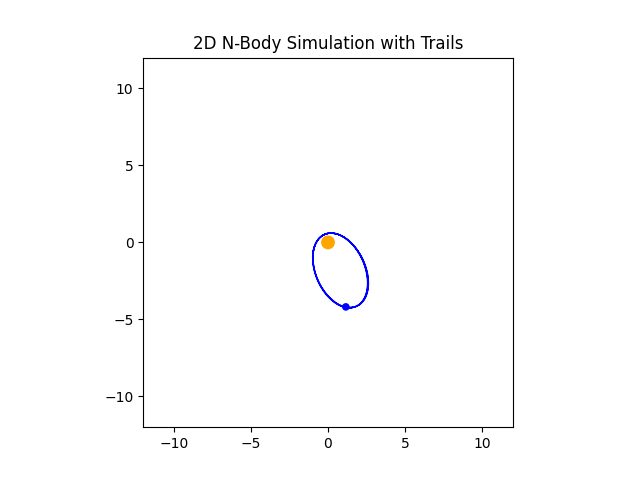
\includegraphics[width=0.6\linewidth]{2_body_orbit.png}
    \caption{Two-body test: a stationary massive body (orange) and a lighter body (blue) in orbit.}
    \label{fig:two_body_orbit}
\end{figure}
The plot in Figure~\ref{fig:two_body_orbit} was obtained by setting the configuation file read by \emph{serial\_testing.c}, as follows:
\begin{itemize}
    \item Body~0 (massive): $m = 1.0$, initial position $(0,0,0)$, initial velocity $(0,0,0)$;
    \item Body~1 (light): $m = 3\times 10^{-6}$, initial position $(-1,-1,0)$, initial velocity $(0,6,0)$.
\end{itemize}
The time step was set to $\Delta t = 0.01$, and the simulation was run for $T=2000$ steps.

A second test was performed using a larger set of bodies, inspired by a simplified solar system model.  
Figure~\ref{fig:long_solar_system} shows the result of a longer simulation run with $T = 2000$ time steps.
\begin{figure}[H]
    \centering
    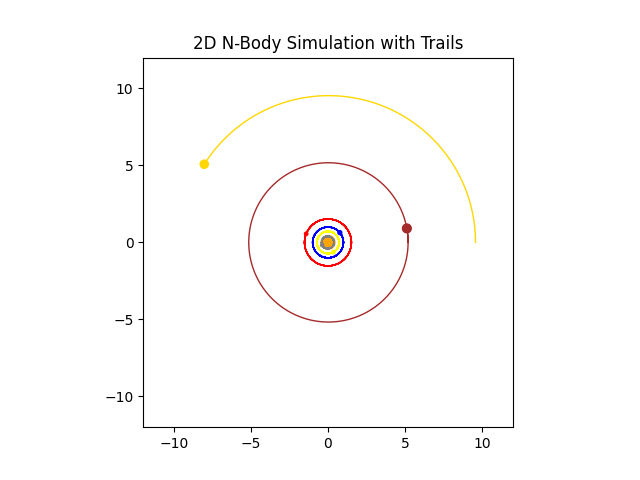
\includegraphics[width=0.6\linewidth]{long_solar_system.png}
    \caption{Solar system test: all the planets revolves steadily around the central star.}
    \label{fig:long_solar_system}
\end{figure}
Throughout the simulation, no planet escaped its orbit, indicating that the numerical integration preserved stability over time.  
Moreover, bodies at different distances from the central mass exhibited the expected orbital periods, and gravitational interactions between planets did not cause unphysical divergence.

These qualitative observations confirm that the combination of the direct gravitational computation and the chosen symplectic integrator (\S\ref{subsec:num_int}) yields a physically plausible evolution, even over longer durations.
  
The parameters used to produce Figure~\ref{fig:long_solar_system} are reported in Appendix~\ref{appendix:solar_params}.

\subsubsection{Random Initialization}
The standard version of the serial application initialized the simulated system randomly. This makes simpler doing experiments with a large quantities of bodies: the program receives the number of bodies from the user through the command-line.
It is worth noticing the use into the inizialization routine of the function \emph{rand\_uniform}.
\begin{lstlisting}
double rand_uniform(unsigned int *seed, double min, double max) {
    return min + (max - min) * ((double)rand_r(seed) / RAND_MAX);
}
\end{lstlisting}
Using a seed allows to have random reproducible inizializations since a seed determines the beginning of the pseudo-random sequence of values and furthermore the calling of \emph{rand\_r(seed)} ensures that each different processes who may running the application use the same seed. The latter will be crucial when comparing the results with the parallel application.
Please also notice that in \emph{rand\_uniform} function we also normalize what \emph{rand\_r(seed)} returns and bounds that number to an arbitrary range and that RNG values are drawn from an uniform distribution in order to avoid directional or positional biases.

In our experiments the interval $\left(-1.0, 1.0\right)$ has been forced to focus on the gravitational interaction.


\subsubsection{Performance Analysis}
\label{sec:performance_analysis}
In subsection~\ref{subsec:time_complexity}, it was shown that the time complexity of the serial algorithm is $O(N^2)$.  
To evaluate whether this theoretical estimate holds in practice, the C implementation was executed eight times with the number of bodies $N$ increasing from $100$ to $12\,800$.  
For all runs, the number of simulation steps was fixed at $T = 100$, the time step size at $\Delta t = 0.01$, and the gravitational constant at $G = 39.47$.  

Execution time was measured using the \emph{clock} function from the C standard library (\texttt{time.h}).  

The tests were conducted on a machine whose detailed specifications are reported in Appendix~\ref{appendix:machine_specs}.

\begin{figure}[H]
    \centering
    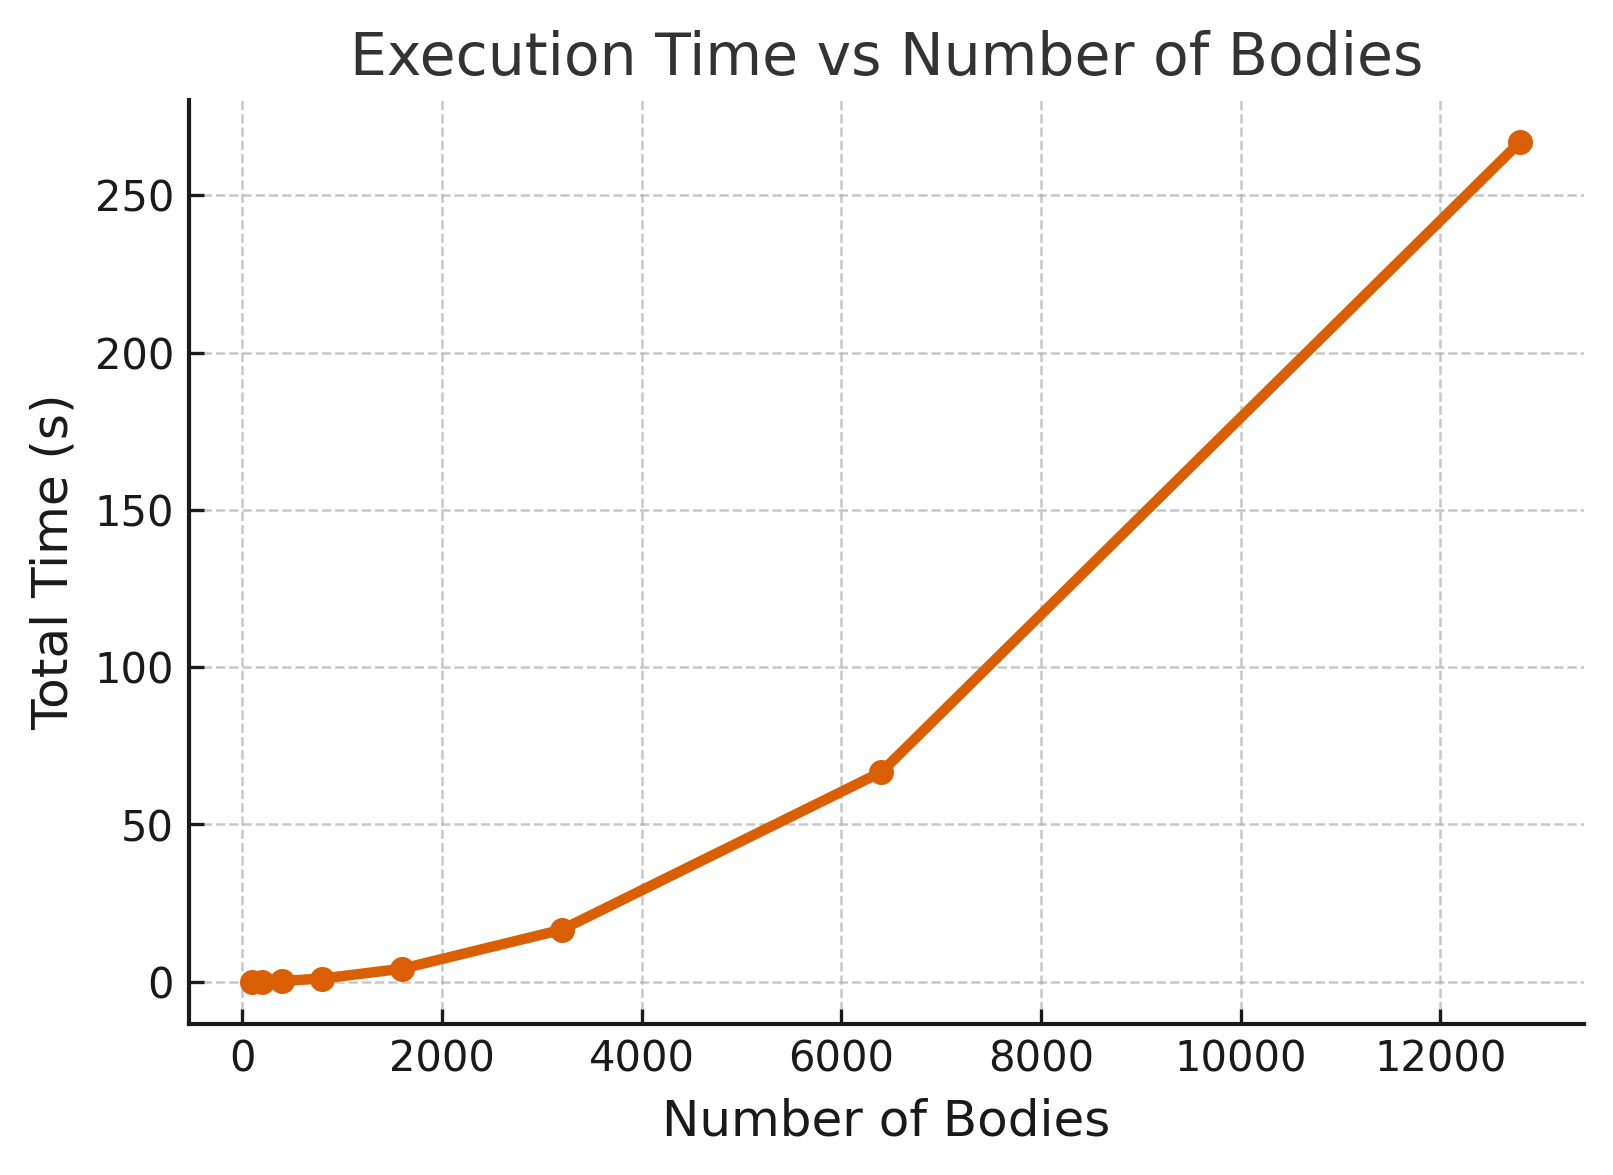
\includegraphics[width=0.6\linewidth]{ex_time_vs_bodies.png}
    \caption{Execution time as a function of the number of bodies $N$.}
    \label{fig:ex_time}
\end{figure}
As expected the running time has a non-linear relationship with the number of bodies as can be seen in Figure \ref{fig:ex_time}.

The log-log plot in Figure \ref{fig:logex_time} reveals an approximately straight line, indicating a power-law relationship, i.e., a quantity varies with the power of another, suggesting a time complexity around $O(N^2)$.

\begin{figure}[H]
    \centering
    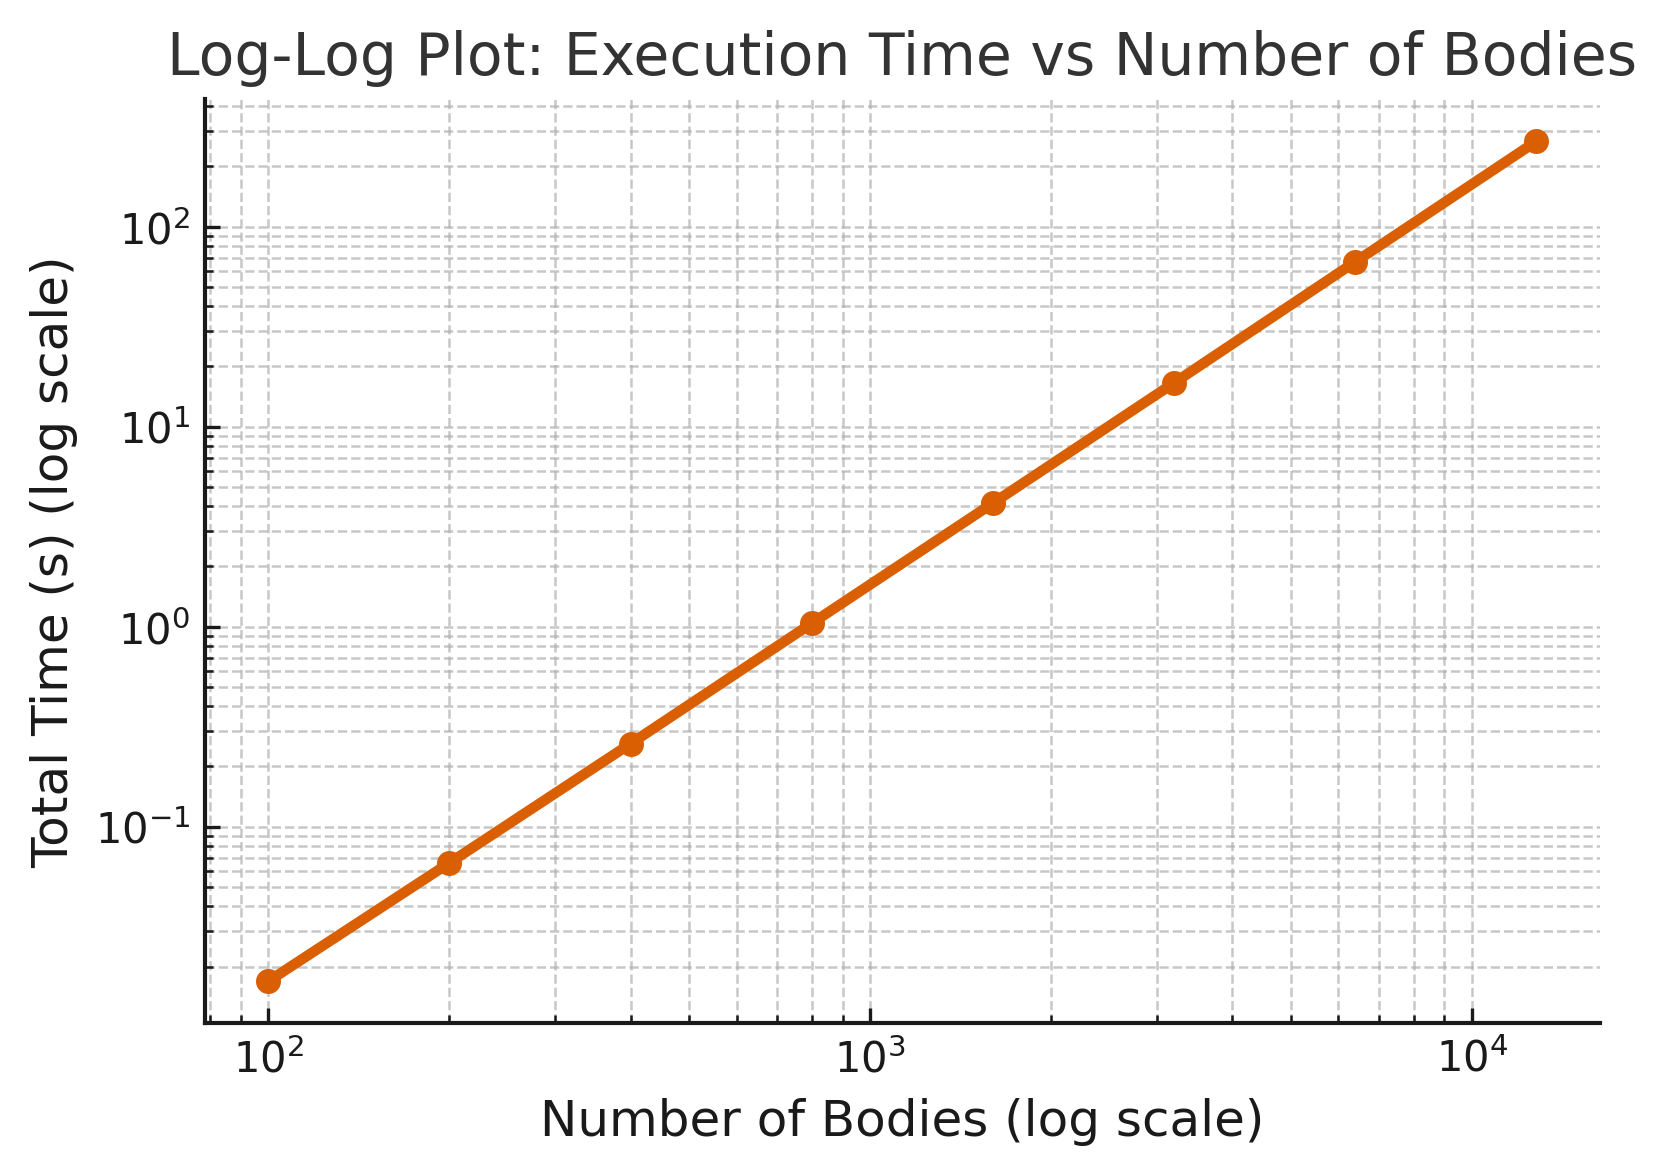
\includegraphics[width=0.6\linewidth]{logex_time_vs_logbodies.png}
    \caption{Log-log plot of execution time vs.\ number of bodies, revealing a power-law relationship.}
    \label{fig:logex_time}
\end{figure}
The raw measurements used to generate Figures~\ref{fig:ex_time} and~\ref{fig:logex_time} are reported in Appendix~\ref{appendix:serial_times}.

Since the empirical results confirmed that the time complexity of the C program is $O(N^2)$, it is worth recalling the reasoning presented in subsection~\ref{subsec:time_complexity}: the overall time complexity is dominated by the \emph{Compute accelerations} algorithm~\ref{alg:inner_loop}, as the other components of the serial algorithm involve only a single loop over the $N$ bodies ($N$ being the problem size).
This implies that the execution time is mainly due to the \texttt{compute\discretionary{}{}{}Accelerations()} function.

To verify this, the C code was compiled with profiling enabled, and the \emph{gprof} profiler 
was used to produce a performance report. The main results are presented in 
Appendix~\ref{appendix:gprof_results}.
As predicted, \texttt{computeAccelerations()} dominates the runtime (98.49\%), confirming it is the primary bottleneck of the serial implementation.

It is also insightful to analyze performance from a hardware perspective. The built-in Linux profiler \emph{perf} was used for this purpose.
The results of the \emph{perf} profiler are reported in Appendix~\ref{appendix:perf_results}.

Since \texttt{compute\discretionary{}{}{}Accelerations()} keeps the CPU busy for the vast majority of execution time, these measurements can be safely attributed to this function.

The very low branch-miss rate ($0.06\%$) indicates that the control flow within the inner loop is highly predictable. Furthermore, the low percentage of frontend idle cycles ($0.14\%$) confirms that the workload is highly CPU-bound.
The measured instructions-per-cycle (IPC) of $2.43$ corresponds to a cycles-per-instruction (CPI) of approximately $0.41$, meaning that on average each instruction is retired in less than one clock cycle. This is likely due to the microarchitecture of the test machine, which can exploit multiple execution pipelines, out-of-order execution, minimal memory stalls and compiler optimizations.

The computer can do so because there are very little data dependencies present in the \texttt{compute\discretionary{}{}{}Accelerations()} function: to compute the accelerations it is required to produce first the positions.

On the other hand is crucial to notice that the inner loop iterations are independent from one another, i.e, they could be overlapped.
This means, of course that loop unrolling can be applied, but more importantly that the loop iterations can be distributed accross processes.

%
%Parallel applications
%

\appendix


\section[Simulation Parameters (Solar System)]{Simulation Parameters for the Solar System Test}
\label{appendix:solar_params}

The following configuration was used for the simulation shown in Figure~\ref{fig:long_solar_system}:

\begin{verbatim}
39.4784176 10 20000 0.001
1.0
0 0 0
0 0 0
3.00e-6
0.39 0 0
0 10.2 0
3.26e-7
0.72 0 0
0 7.4 0
3.00e-6
1.0 0 0
0 6.28 0
3.32e-7
1.52 0 0
0 5.1 0
9.50e-4
5.2 0 0
0 2.75 0
2.86e-4
9.58 0 0
0 2.03 0
4.36e-5
19.2 0 0
0 1.43 0
5.15e-5
30.1 0 0
0 1.14 0
1.02e-8
39.5 0 0
0 1.0 0
\end{verbatim}

Where the first line specifies:
\begin{itemize}
    \item Gravitational constant $G$
    \item Number of bodies $N$
    \item Number of steps $T$
    \item Time step $\Delta t$
\end{itemize}
and each body is defined by: mass, initial $(x, y, z)$ position, and initial $(v_x, v_y, v_z)$ velocity.

\section[Machine Specifications]{Machine Specifications}
\label{appendix:machine_specs}
\begin{tabular}{ll}
\toprule
Architecture & x86\_64 \\
CPU Model & AMD Ryzen 5 5625U with Radeon Graphics (12 threads, 6 cores) \\
Base/Max Clock & 2.3 GHz / 4.388 GHz \\
L1 Cache & 192 KiB (6 instances) \\
L2 Cache & 3 MiB (6 instances) \\
L3 Cache & 16 MiB (1 instance) \\
Memory & 8 GB DDR4 \\
OS & Ubuntu 22.04.5 LTS, 64-bit \\
Compiler & \texttt{gcc} 11.4.0 with \texttt{-O2} optimization \\
\bottomrule
\end{tabular}

\section{Serial Implementation Timing Data}
\label{appendix:serial_times}
The following table reports the execution times (in seconds) measured for the performance analysis in Section~\ref{sec:performance_analysis}.

\begin{table}[H]
    \centering
    \begin{tabular}{r r}
        \toprule
        \textbf{$N$ (bodies)} & \textbf{Execution time (s)} \\
        \midrule
        100 & 0.012 \\
        200 & 0.049 \\
        400 & 0.198 \\
        800 & 0.796 \\
        1600 & 3.187 \\
        3200 & 12.732 \\
        6400 & 50.902 \\
        12800 & 203.671 \\
        \bottomrule
    \end{tabular}
    \caption{Execution times used to generate Figures~\ref{fig:ex_time} and~\ref{fig:logex_time}.}
    \label{tab:serial_times}
\end{table}

\section{Profiling Results}
\label{appendix:profiling_results}
This appendix reports profiling data for the serial C implementation.
Two profiling tools were used:
\begin{itemize}
    \item GNU \emph{gprof}, to obtain a function-level breakdown of execution time.
    \item Linux \emph{perf}, to collect low-level CPU performance metrics.
\end{itemize}

\subsection{gprof Flat Profile (Summary)}
\label{appendix:gprof_results}
The program was compiled with the \texttt{-pg} flag and executed under the same settings used in the performance analysis (\S\ref{sec:performance_analysis}) with the exception of $N = 10000$. The resulting \texttt{gmon.out} file was processed with:
\begin{verbatim}
gprof serial gmon.out > profiling_report.txt
\end{verbatim}
\begin{table}[H]
\centering
\label{tab:gprof_summary}
\begin{tabular}{lrrr}
\toprule
\textbf{Function} & \textbf{\% Time} & \textbf{Self (s)} & \textbf{Calls}  \\
\midrule
\texttt{computeAccelerations} & 98.49 & 150.54 & 100 \\
\texttt{\_init}               &  1.49 &   2.28 & --- \\
\texttt{computeVelocities}    &  0.01 &   0.02 & 100 \\
\texttt{logPositions}         &  0.01 &   0.01 & 101 \\
\texttt{rand\_uniform}        &  0.00 &   0.00 & 60000 \\
\texttt{computePositions}     &  0.00 &   0.00 & 100 \\
\texttt{simulate}             &  0.00 &   0.00 & 100 \\
\texttt{initiateSystem}       &  0.00 &   0.00 & 1   \\
\bottomrule
\end{tabular}
\caption{Distribution of execution time by function (gprof flat profile).}
\end{table}
Please note that the \texttt{\_init} function is not part of the N-body program; it is automatically inserted by the C runtime environment during the executable’s startup sequence to perform system-level 
initializations before \texttt{main()} is called.


\subsection{perf Results}
\label{appendix:perf_results}
The profiling command used was:
\begin{verbatim}
perf stat ./serial 12800
\end{verbatim}
\begin{table}[H]
\centering
\label{tab:perf_summary}
\begin{tabular}{l r}
\toprule
\textbf{Metric} & \textbf{Value} \\
\midrule
Task-clock & $268.400$ ms \\
CPU Utilization & $1.000$ CPUs \\
Context-switches & $933$ ($3.48$/s) \\
CPU Migrations & $194$ ($0.72$/s) \\
Page-faults & $316$ ($1.18$/s) \\
Cycles & $1.165 \times 10^{9}$ ($4.341$ GHz) \\
Stalled-cycles-frontend & $1.590 \times 10^{6}$ ($0.14\%$ frontend idle) \\
Instructions & $2.837 \times 10^{9}$ ($2.43$ IPC) \\
Branches & $1.152 \times 10^{8}$ \\
Branch-misses & $7.05 \times 10^{7}$ ($0.06\%$ of all branches) \\
Elapsed time & $268.410$ s \\
User time & $268.398$ s \\
System time & $0.002$ s \\
\bottomrule
\end{tabular}
\caption{\texttt{perf} summary for serial execution with $N = 12\,800$.}
\end{table}





\bibliographystyle{IEEEtran} %I had to install a package through the package manager to use 'IEEEtran'.
\bibliography{refs} 
\end{document}
